\documentclass[t, 10pt]{beamer}
%%\documentclass[t,handout]{beamer}

\usepackage{graphicx}
\usepackage{epsfig}
\usepackage{psfrag}
\usepackage[english]{babel}
\usepackage{color}
\usepackage{natbib}

%Mathematics packages
\usepackage{amsmath}
\usepackage{mathrsfs}
\usepackage{amsfonts}
\usepackage{enumerate}

\graphicspath{{./images/}} % Figures path - used in graphicx

\selectcolormodel{cmyk}

\mode<presentation>

%THEMES - Please refer to these chapters in the beamer documentation.
% Presentation themes : Chapter 15
% Color themes : Chapter 17
% Font themes : Chapter 18


\usetheme{Pittsburgh}
\usecolortheme{orchid}
\usefonttheme{default}

\setbeamertemplate{bibliography item}[text]
\setbeamercovered{transparent=7}

%---------------------------Title frame definition------------------------------------- 

\title{A Domain Specific Language for Usage Management}
\author [Chris]{Christopher C. Lamb, Pramod A. Jamkhedkar, Mathew P. Bohnsack, Viswanath Nandina, Gregory L. Heileman}
\institute[University of New Mexico]{
\inst {}Department of Electrical and Computer Engineering\\
University of New Mexico}
\date{October 21, 2011}
\titlegraphic{
\begin{figure} 
\includegraphics[width = 7cm]{UNM}
\end{figure}}

% Delete this, if you do not want the table of contents to pop up at
% the beginning of each subsection:
%\AtBeginSubsection[]
%{
%  \begin{frame}<beamer>
%    \frametitle{Outline}
%     \tableofcontents[currentsection,currentsubsection]
%  \end{frame}
%}

\begin{document}

\begin{frame}
\titlepage
\end{frame}

% This command will make the logo appear on all frames excluding the title frame.
\logo {\includegraphics[width = 2.5cm]{UNM}}

\begin{frame}[t]
\frametitle{Outline}
\tableofcontents 
\end{frame}

\section{Introduction}
\begin{frame}[t]
\frametitle{Introduction}
Intro content
\end{frame}

\section{Design}
\begin{frame}[t]
\frametitle{Design --- Notional Use}
\begin{columns}[t]
\column{.5\textwidth}
Notional Use:
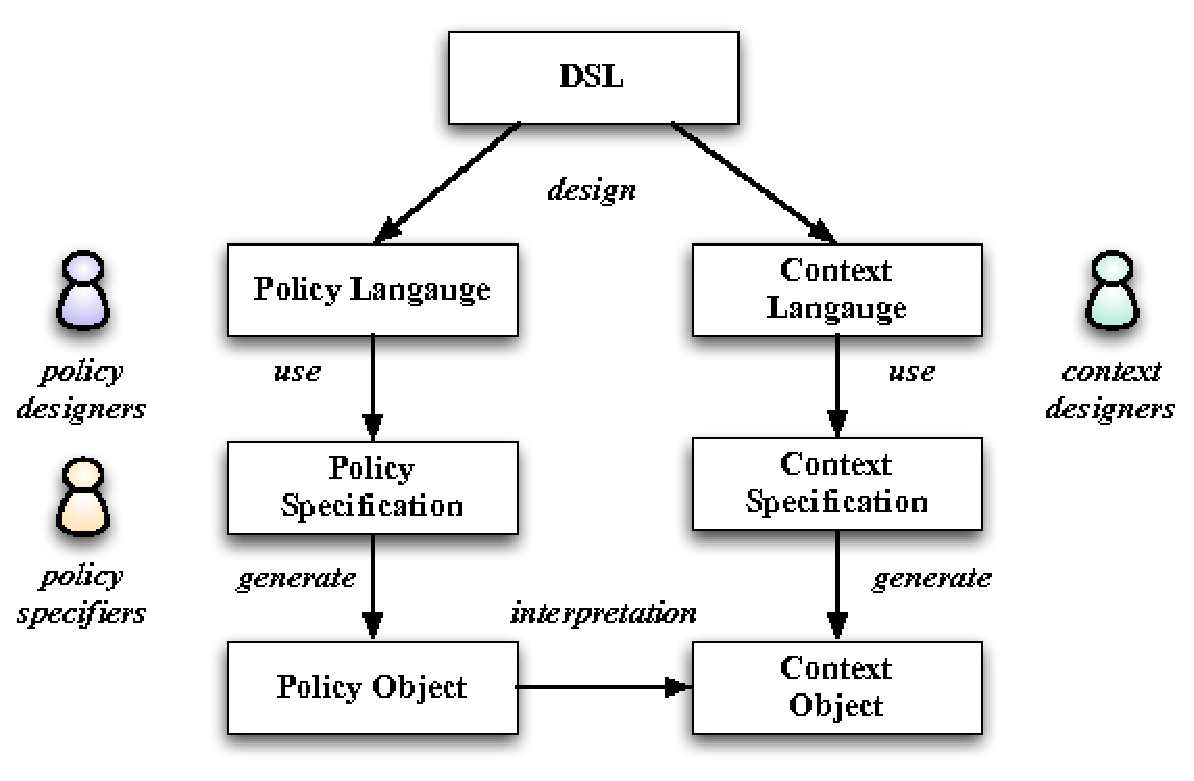
\includegraphics[width=2.4in]{players}
\begin{itemize}
\item<2-> \textit{DSL} --- Domain specific language
\item<3-> \textit{Policy Language} --- Language elements specific to \textit{policy}
\end{itemize}
\column{.5\textwidth}
\begin{itemize}
\item<4-> \textit{Context Language} --- Language elements specific to \textit{context}
\item<5-> \textit{Policy Specification} --- Actual specification of policy
\item<6-> \textit{Context Specification} --- Specification of context requirements
\item<7-> \textit{Policy Object} --- An object embodying policy created from the DSL
\item<8-> \textit{Context Object} --- An object containing context information used by the policy object
\end{itemize}
\end{columns}
\end{frame}

\begin{frame}{t}
\frametitle{Design --- Use Cases}
\begin{columns}[t]
\column{.5\textwidth}
Use Cases:
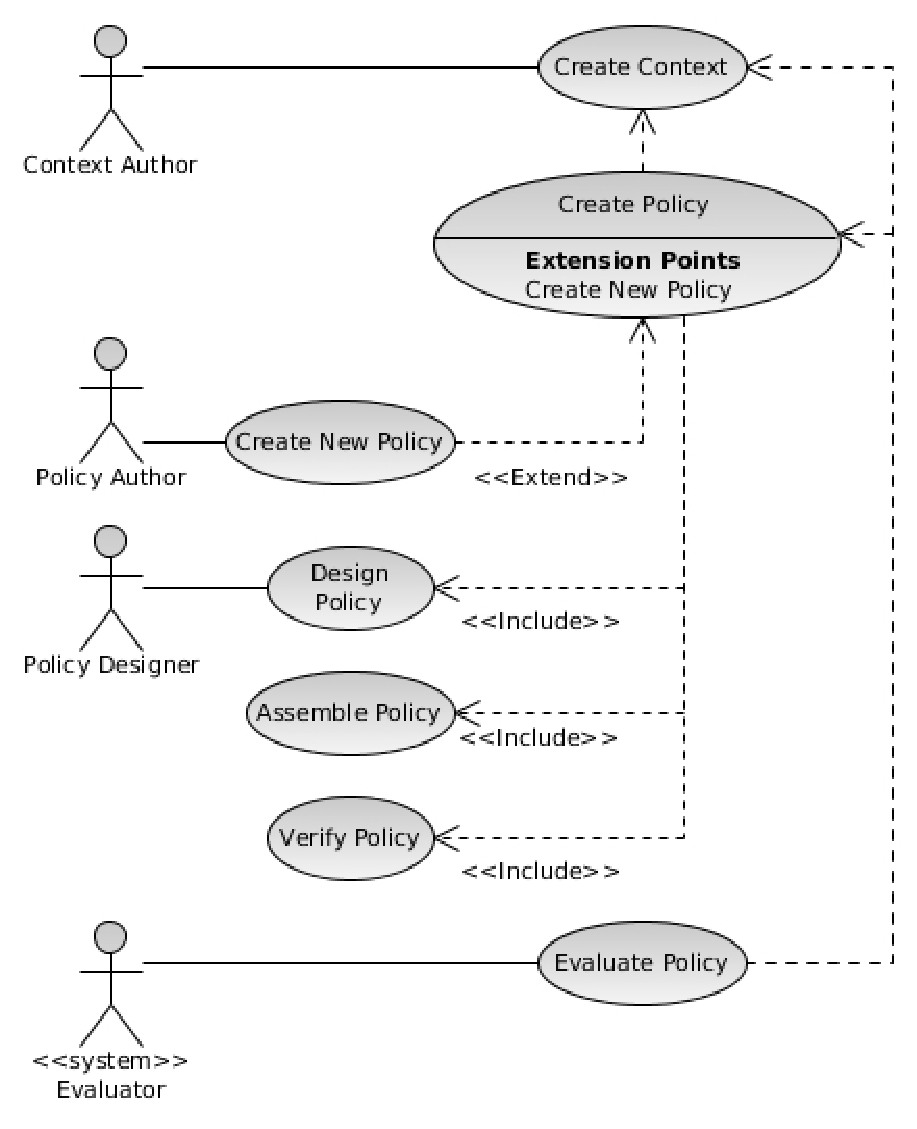
\includegraphics[width=2.3in]{use-cases}
\column{.5\textwidth}
\begin{itemize}
\item<2-> \textit{Create Context} ---
\item<3-> \textit{Create Policy} ---
\item<4-> \textit{Evaluate Policy} ---
\end{itemize}
\end{columns}
\end{frame}

\begin{frame}{t}
\frametitle{Design --- Domain Model}
\begin{columns}[t]
\column{.5\textwidth}
Domain Model:
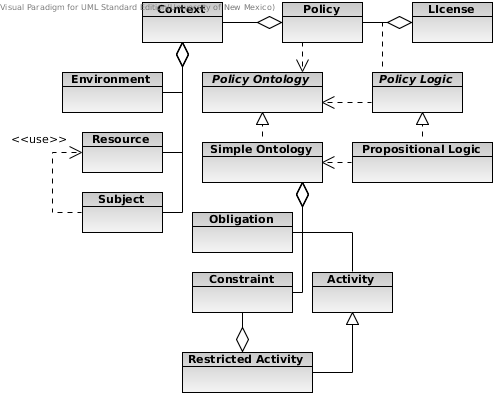
\includegraphics[width=2.3in]{ontology}
\column{.5\textwidth}
\pause
The \textit{Runtime} accesses and activates a \textit{policy} and manages a \textit{context} to which the policy is given a reference.
\newline
\newline
\pause
The \textit{context} has access to information about the \textit{environment}, \textit{resource} managed, and the \textit{subject} using the \textit{resource}. 
\newline
\newline
\pause
Interactions are described by specific \textit{usage semantics} embodied in the \textit{policy}.
\end{columns}
\end{frame}

\begin{frame}{t}
\frametitle{Design --- Usage Semantics}
\begin{columns}[t]
\column{.5\textwidth}
\column{.5\textwidth}
\end{columns}
\end{frame}

\section{Implementation}
\begin{frame}[t]
\frametitle{Introduction}
Intro content
\end{frame}

\section{Application}
\begin{frame}[t]
\frametitle{Introduction}
Intro content
\end{frame}

\begin{frame}{t}
\frametitle{Sample --- Thing}
\begin{columns}[t]
\column{.5\textwidth}
\column{.5\textwidth}
\end{columns}
\end{frame}

\end{document}

